\chapter{Appendix}
\label{sec:appendix}
\raggedbottom

\section{XPS of QA on the Ag(100) with multilayer coverages}


\section{LEED patterns of QA on the Ag(100) surface}

\begin{figure}[H]
    \centering
    \subfloat[\Ac{POL} $\alpha$-phase]{%
        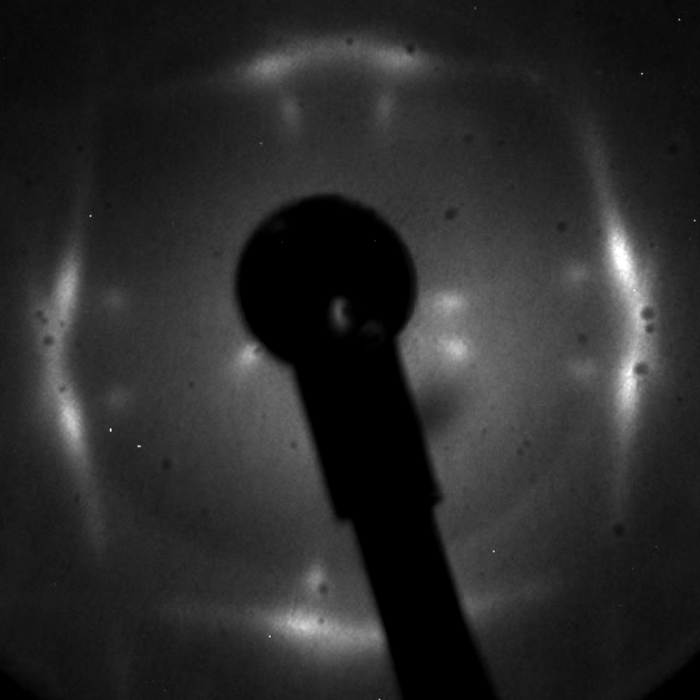
\includegraphics[width=0.45\textwidth]{images/vertiefer/LEED/LEED-alpha-25.5eV.png}
    }
    \hspace{0.05\textwidth}
    \subfloat[Commensurate $\beta$-phase]{%
        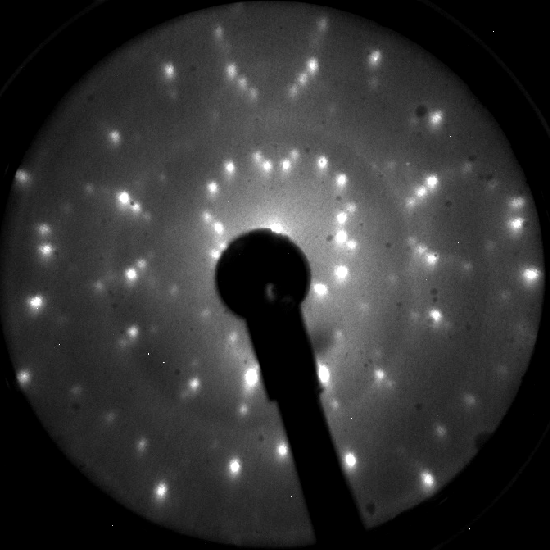
\includegraphics[width=0.45\textwidth]{images/vertiefer/LEED/LEED-beta-25.5eV.png}
    }
    \caption{\Ac{LEED} patterns for the $\alpha$- and the $\beta$-phase at 25.5~\si{eV} taken at the I09 beamline of the Diamond Light Source.}
    \label{fig:LEED}
\end{figure}

\newpage
\section*{List of abbreviations}
\addcontentsline{toc}{section}{List of abbreviations}

\begin{acronym}
    \acro{BE}[BE]{binding energy}
    \acro{fcc}[fcc]{face-centered cubic}
    \acro{FWHM}[FWHM]{full width at half maximum}
    \acro{LEED}[LEED]{low energy electron diffraction}
    \acro{ML}[ML]{monolayer}
    \acro{NIXSW}[NIXSW]{normal incidence x-ray standing wavefield absorption}
    \acro{OFET}[OFET]{organic field-effect transistor}
    \acro{OLED}[OLED]{organic light-emitting diode}
    \acro{OPV}[OPV]{organic photovoltaic}
    \acro{POL}[POL]{point-on-line}
    \acro{QA}[QA]{quinacridone}
    \acro{SPA-LEED}[SPA-LEED]{spot profile analysis low energy electron diffraction}
    \acro{STM}[STM]{scanning tunneling microscopy}
    \acro{UHV}[UHV]{ultra-high vacuum}
    \acro{XPS}[XPS]{x-ray photoelectron spectroscopy}
\end{acronym}

\acrodefplural{BE}{binding energies}



